\documentclass[14pt]{extbook}
\usepackage{multicol, enumerate, enumitem, hyperref, color, soul, setspace, parskip, fancyhdr} %General Packages
\usepackage{amssymb, amsthm, amsmath, latexsym, units, mathtools} %Math Packages
\everymath{\displaystyle} %All math in Display Style
% Packages with additional options
\usepackage[headsep=0.5cm,headheight=12pt, left=1 in,right= 1 in,top= 1 in,bottom= 1 in]{geometry}
\usepackage[usenames,dvipsnames]{xcolor}
\usepackage{dashrule}  % Package to use the command below to create lines between items
\newcommand{\litem}[1]{\item#1\hspace*{-1cm}\rule{\textwidth}{0.4pt}}
\pagestyle{fancy}
\lhead{Progress Quiz 7}
\chead{}
\rhead{Version A}
\lfoot{6523-2736}
\cfoot{}
\rfoot{test}
\begin{document}

\begin{enumerate}
\litem{
Find the equation of the line described below. Write the linear equation as $ y=mx+b $ and choose the intervals that contain $m$ and $b$.\[ \text{Parallel to } 3 x - 4 y = 14 \text{ and passing through the point } (-10, 8). \]\begin{enumerate}[label=\Alph*.]
\item \( m \in [-0.2, 0.95] \hspace*{3mm} b \in [-21.5, -14.5] \)
\item \( m \in [-0.2, 0.95] \hspace*{3mm} b \in [18, 19] \)
\item \( m \in [-0.2, 0.95] \hspace*{3mm} b \in [15.5, 17.5] \)
\item \( m \in [-1.15, -0.72] \hspace*{3mm} b \in [-3.5, 2.5] \)
\item \( m \in [0.89, 2.2] \hspace*{3mm} b \in [15.5, 17.5] \)

\end{enumerate} }
\litem{
First, find the equation of the line containing the two points below. Then, write the equation as $ y=mx+b $ and choose the intervals that contain $m$ and $b$.\[ (-7, -9) \text{ and } (11, -11) \]\begin{enumerate}[label=\Alph*.]
\item \( m \in [-0.16, 0.02] \hspace*{3mm} b \in [6.7, 11.8] \)
\item \( m \in [-0.16, 0.02] \hspace*{3mm} b \in [-10.8, -7.2] \)
\item \( m \in [-0.16, 0.02] \hspace*{3mm} b \in [-4.7, 0.7] \)
\item \( m \in [-0.16, 0.02] \hspace*{3mm} b \in [-24.7, -19.3] \)
\item \( m \in [-0.02, 0.33] \hspace*{3mm} b \in [-15.4, -11.6] \)

\end{enumerate} }
\litem{
Solve the equation below. Then, choose the interval that contains the solution.\[ -6(-4x -5) = -7(-17x -3) \]\begin{enumerate}[label=\Alph*.]
\item \( x \in [0.09, 0.34] \)
\item \( x \in [0.29, 0.55] \)
\item \( x \in [-0.42, -0.13] \)
\item \( x \in [-0.6, -0.5] \)
\item \( \text{There are no real solutions.} \)

\end{enumerate} }
\litem{
Solve the linear equation below. Then, choose the interval that contains the solution.\[ \frac{6x + 5}{7} - \frac{9x + 5}{6} = \frac{-4x + 7}{3} \]\begin{enumerate}[label=\Alph*.]
\item \( x \in [1.9, 3.4] \)
\item \( x \in [3.5, 5] \)
\item \( x \in [0.1, 1.8] \)
\item \( x \in [9.1, 10.5] \)
\item \( \text{There are no real solutions.} \)

\end{enumerate} }
\litem{
Write the equation of the line in the graph below in Standard form $Ax+By=C$. Then, choose the intervals that contain $A, B, \text{ and } C$.
\begin{center}
    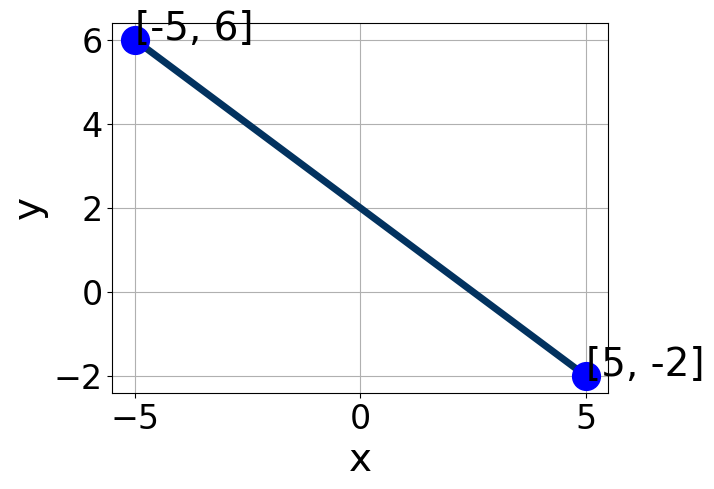
\includegraphics[width=0.5\textwidth]{../Figures/linearGraphToStandardCopyA.png}
\end{center}
\begin{enumerate}[label=\Alph*.]
\item \( A \in [1.6, 2.85], \hspace{3mm} B \in [-6.5, -4.6], \text{ and } \hspace{3mm} C \in [-10, -3] \)
\item \( A \in [-2.55, -0.55], \hspace{3mm} B \in [-6.5, -4.6], \text{ and } \hspace{3mm} C \in [-10, -3] \)
\item \( A \in [0.22, 1.05], \hspace{3mm} B \in [-0.6, 2.2], \text{ and } \hspace{3mm} C \in [1, 4] \)
\item \( A \in [0.22, 1.05], \hspace{3mm} B \in [-1.8, 0.6], \text{ and } \hspace{3mm} C \in [-3, 1] \)
\item \( A \in [1.6, 2.85], \hspace{3mm} B \in [4, 5.6], \text{ and } \hspace{3mm} C \in [9, 14] \)

\end{enumerate} }
\litem{
Solve the linear equation below. Then, choose the interval that contains the solution.\[ \frac{-8x + 5}{7} - \frac{-6x -5}{2} = \frac{5x -7}{3} \]\begin{enumerate}[label=\Alph*.]
\item \( x \in [-2.88, -0.88] \)
\item \( x \in [-1.21, 4.79] \)
\item \( x \in [-92.25, -86.25] \)
\item \( x \in [-30.12, -28.12] \)
\item \( \text{There are no real solutions.} \)

\end{enumerate} }
\litem{
First, find the equation of the line containing the two points below. Then, write the equation as $ y=mx+b $ and choose the intervals that contain $m$ and $b$.\[ (3, -10) \text{ and } (11, -11) \]\begin{enumerate}[label=\Alph*.]
\item \( m \in [-0.14, -0.04] \hspace*{3mm} b \in [-13.98, -12.81] \)
\item \( m \in [-0.14, -0.04] \hspace*{3mm} b \in [-22.43, -21.83] \)
\item \( m \in [-0.09, 0.13] \hspace*{3mm} b \in [-12.54, -12.35] \)
\item \( m \in [-0.14, -0.04] \hspace*{3mm} b \in [9.02, 10] \)
\item \( m \in [-0.14, -0.04] \hspace*{3mm} b \in [-9.71, -9.03] \)

\end{enumerate} }
\litem{
Solve the equation below. Then, choose the interval that contains the solution.\[ -8(3x -12) = -6(19x + 14) \]\begin{enumerate}[label=\Alph*.]
\item \( x \in [0.13, 0.18] \)
\item \( x \in [-2.02, -1.91] \)
\item \( x \in [-0.18, -0.04] \)
\item \( x \in [0.05, 0.09] \)
\item \( \text{There are no real solutions.} \)

\end{enumerate} }
\litem{
Write the equation of the line in the graph below in Standard form $Ax+By=C$. Then, choose the intervals that contain $A, B, \text{ and } C$.
\begin{center}
    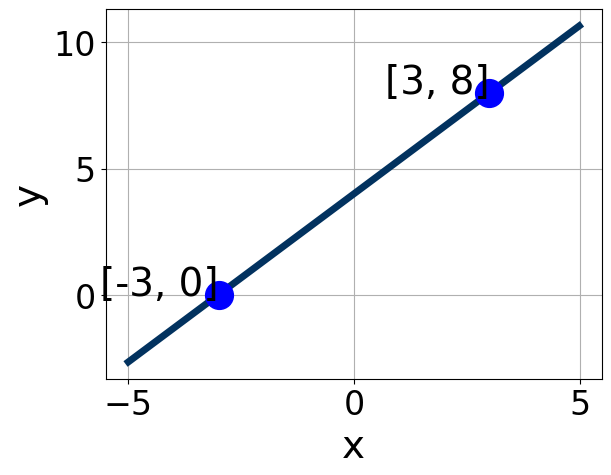
\includegraphics[width=0.5\textwidth]{../Figures/linearGraphToStandardA.png}
\end{center}
\begin{enumerate}[label=\Alph*.]
\item \( A \in [0.4, 3.3], \hspace{3mm} B \in [-2.27, -1.7], \text{ and } \hspace{3mm} C \in [-2.2, -1.64] \)
\item \( A \in [0.4, 3.3], \hspace{3mm} B \in [1.93, 2.73], \text{ and } \hspace{3mm} C \in [1.73, 2.45] \)
\item \( A \in [-2.6, -0.2], \hspace{3mm} B \in [-1.73, -0.39], \text{ and } \hspace{3mm} C \in [-1.83, 0.55] \)
\item \( A \in [-2.6, -0.2], \hspace{3mm} B \in [0.74, 1.42], \text{ and } \hspace{3mm} C \in [0.89, 1.15] \)
\item \( A \in [-6.7, -1.7], \hspace{3mm} B \in [1.93, 2.73], \text{ and } \hspace{3mm} C \in [1.73, 2.45] \)

\end{enumerate} }
\litem{
Find the equation of the line described below. Write the linear equation as $ y=mx+b $ and choose the intervals that contain $m$ and $b$.\[ \text{Parallel to } 3 x - 4 y = 10 \text{ and passing through the point } (3, 3). \]\begin{enumerate}[label=\Alph*.]
\item \( m \in [0.42, 0.77] \hspace*{3mm} b \in [-1.24, -0.55] \)
\item \( m \in [0.42, 0.77] \hspace*{3mm} b \in [-0.4, 0.25] \)
\item \( m \in [1.04, 1.59] \hspace*{3mm} b \in [0.47, 2.22] \)
\item \( m \in [-1.63, -0.69] \hspace*{3mm} b \in [4.45, 6.16] \)
\item \( m \in [0.42, 0.77] \hspace*{3mm} b \in [0.47, 2.22] \)

\end{enumerate} }
\end{enumerate}

\end{document}